
\chapter{Obsah elektronické přílohy}

\dirtree{%
 .1 .
 .2 Firmware.
 .3 IMUnav\_STM\_F00.
 .4 Core.
 .5 AccelCalSolver.
 .6 \dots.
 .5 Inc.
 .6 \dots.
 .5 Src.
 .6 \dots.
 .4 Debug.
 .5 \dots.
 .4 Drivers.
 .5 \dots.
 .4 FATFS.
 .5 \dots.
 .4 Middlewares.
 .5 \dots.
 .4 Release.
 .5 \dots.
 .4 USB\_DEVICE.
 .5 \dots.
 .4 IMUnav\_STM\_F00 Debug.launch.
 .4 IMUnav\_STM\_F00.ioc.
 .4 STM32F446VETX\_FLASH.ld.
 .4 STM32F446VETX\_RAM.ld.
 .2 Hardware.
 .3 IMUnav-library.
 .4 \dots.
 .3 IMUnav\_H00.
 .4 bom.
 .5 ibom.html.
 .4 production.
 .5 \dots.
 .4 ESP32.kicad\_sch.
 .4 GPS.kicad\_sch.
 .4 IMU.kicad\_sch.
 .4 IMU.kicad\_sch-bak.
 .4 IMUnav\_H00.kicad\_dru.
 .4 IMUnav\_H00.kicad\_pcb.
 .4 IMUnav\_H00.kicad\_prl.
 .4 IMUnav\_H00.kicad\_pro.
 .4 IMUnav\_H00.kicad\_sch.
 .4 IMUnav\_H00.kicad\_sch-bak.
 .4 IMUnav\_H00.step.
 .4 Memory.kicad\_sch.
 .4 USB+Power.kicad\_sch.
 .4 User.kicad\_sch.
 .4 fp-info-cache.
 .4 fp-lib-table.
 .4 sym-lib-table.
 .2 Software.
 .3 Matlab.
 .4 C generator.
 .5 codegen.
 .6 lib.
 .7 \dots.
 .6 mex.
 .7 \dots.
 .5 AccelCalSolver.m.
 .5 AccelCalSolver.prj.
 .5 accelCalibration.m.
 .5 gravityFun.m.
 .4 IMUonlyNavigation.m.
 .4 chuzePoByte.csv.
 .4 chuzeVenkuCALB.csv.
 .4 ctverecChuze.csv.
 .4 ctverecChuze2.csv.
 .4 ctverecChuze3CALB.csv.
 .4 ctverecRychlaChuze.csv.
 .4 imuAndGnssInsfilterMARG.m.
 .4 koleckoKolemFEKTUCALB.csv.
 .4 tiltedStationary.csv.
 .3 Python.
 .4 IMUDATA.BIN.
 .4 binDecoder.py.
}

\chapter{Schéma zapojení inerciální jednotky} \label{schemaApp}
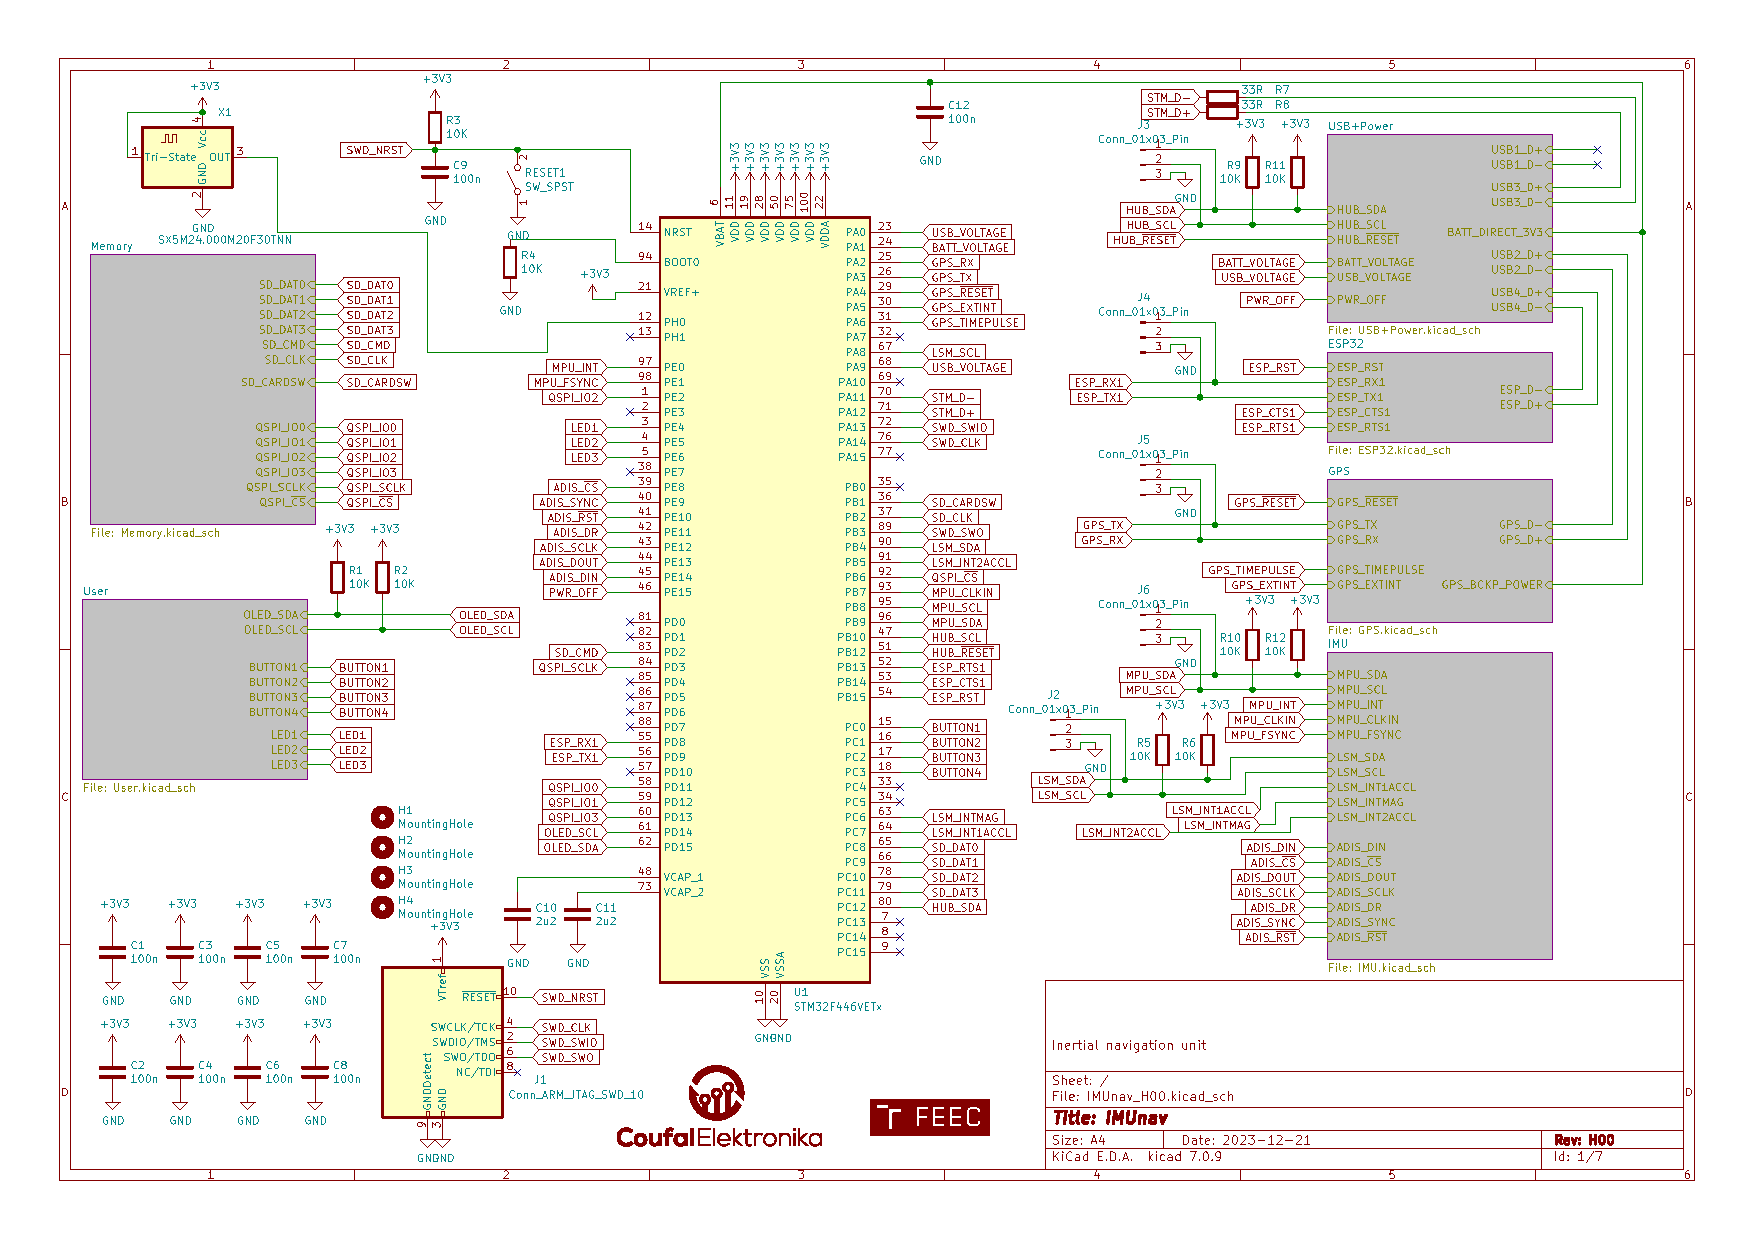
\includegraphics[angle=90, page=1, width=\textwidth]{KiCad/schematic.pdf}

\includegraphics[angle=90, page=2, width=\textwidth]{KiCad/schematic.pdf}

\includegraphics[angle=90, page=3, width=\textwidth]{KiCad/schematic.pdf}

\includegraphics[angle=90, page=4, width=\textwidth]{KiCad/schematic.pdf}

\includegraphics[angle=90, page=5, width=\textwidth]{KiCad/schematic.pdf}

\includegraphics[angle=90, page=6, width=\textwidth]{KiCad/schematic.pdf}

\includegraphics[angle=90, page=7, width=\textwidth]{KiCad/schematic.pdf}

\chapter{Výkres DPS}
\section{Pohled osazení součástek} \label{placementApp}
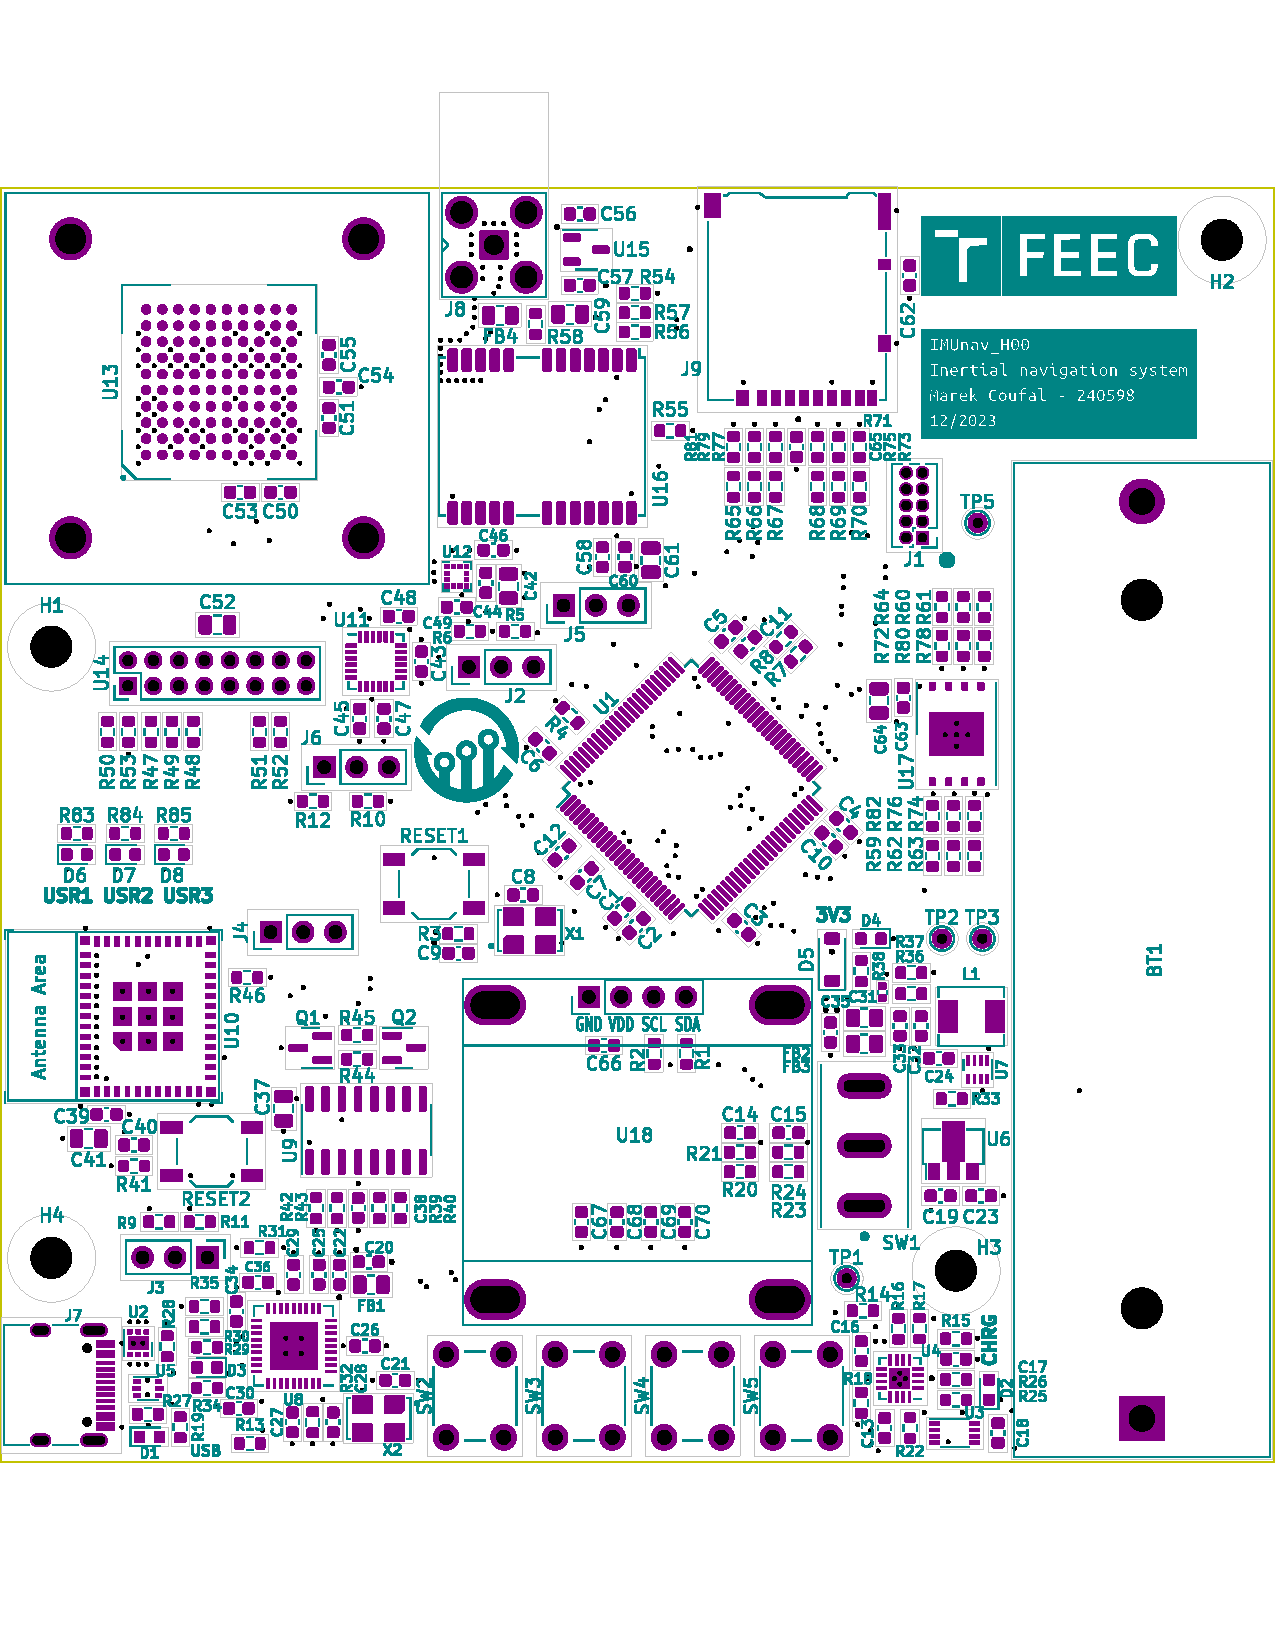
\includegraphics[width=\textwidth]{KiCad/boardTopParts}

\section{Vrchní vrstva mědi DPS} \label{TopApp}
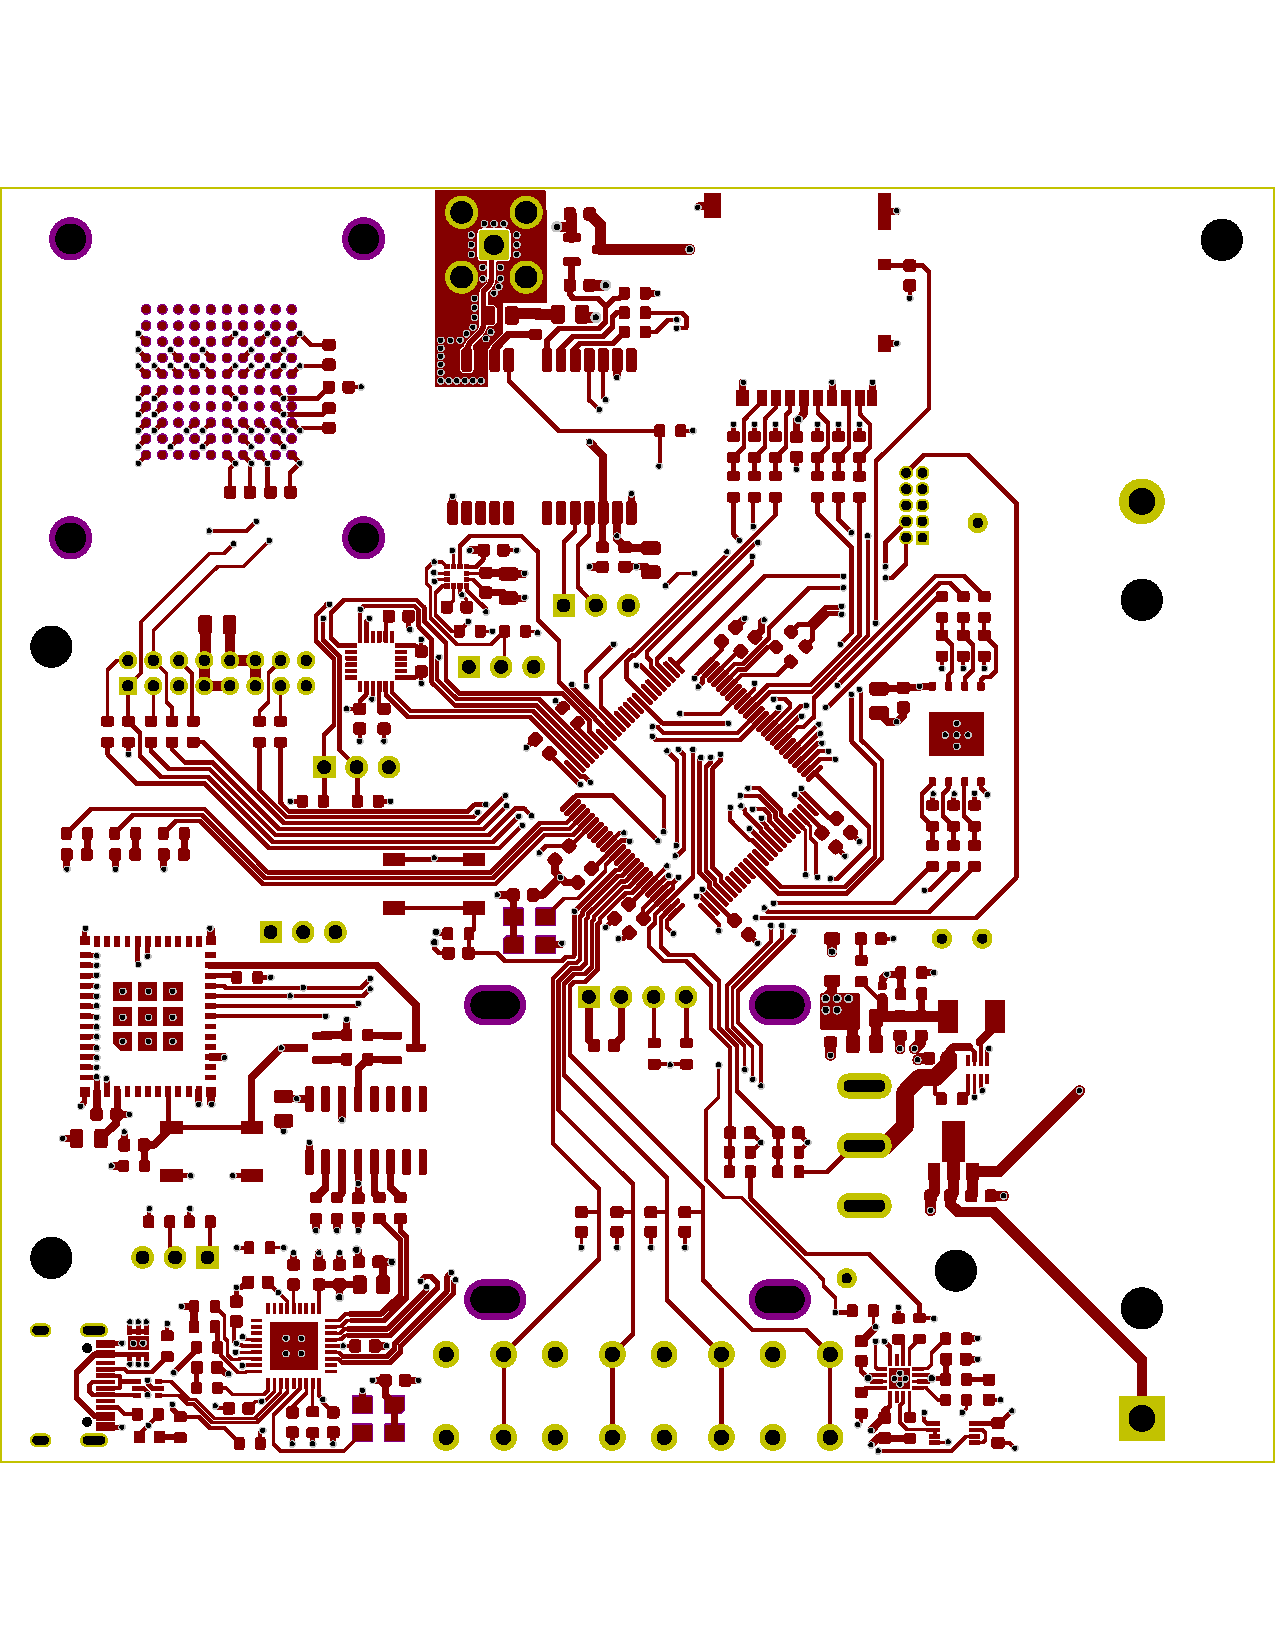
\includegraphics[width=\textwidth]{KiCad/boardF}

\section{Vnitřní vrstva mědi DPS In1}
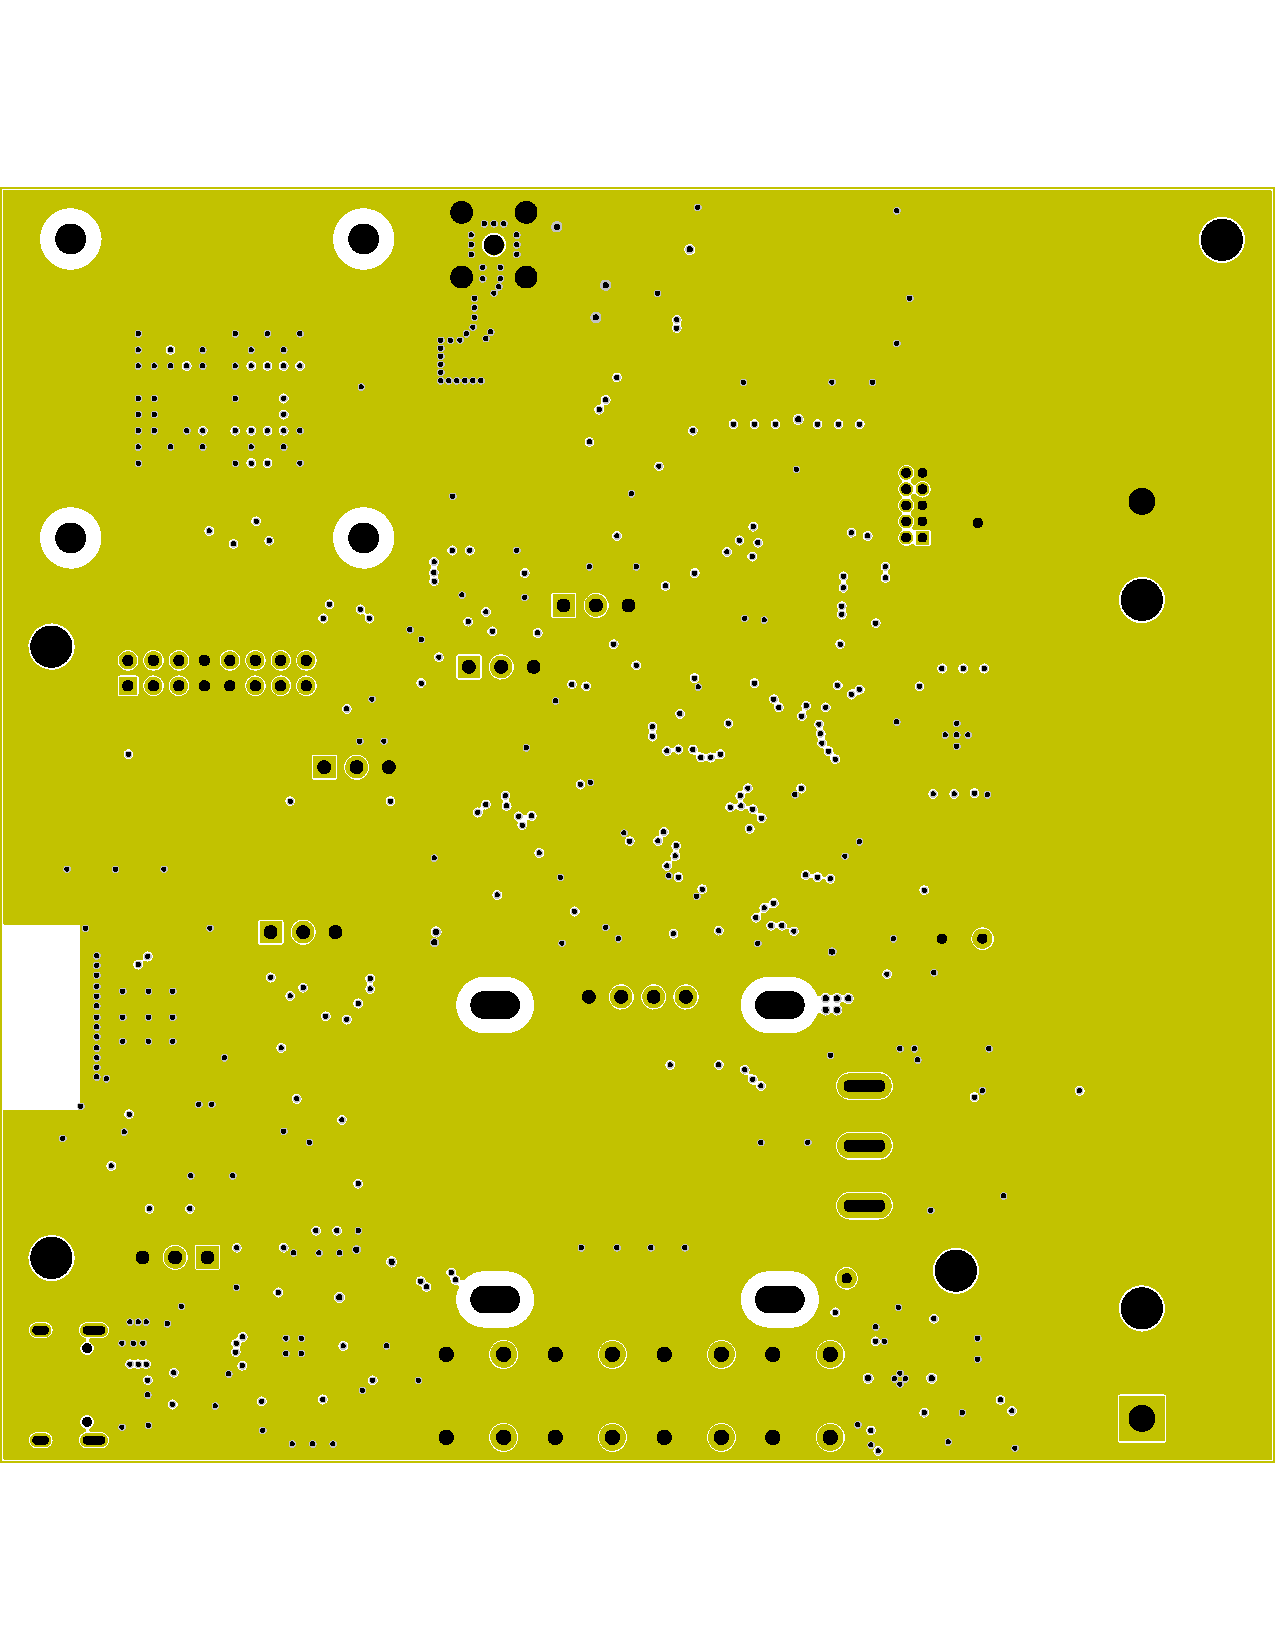
\includegraphics[width=\textwidth]{KiCad/boardIn1}

\section{Vnitřní vrstva mědi DPS In2}
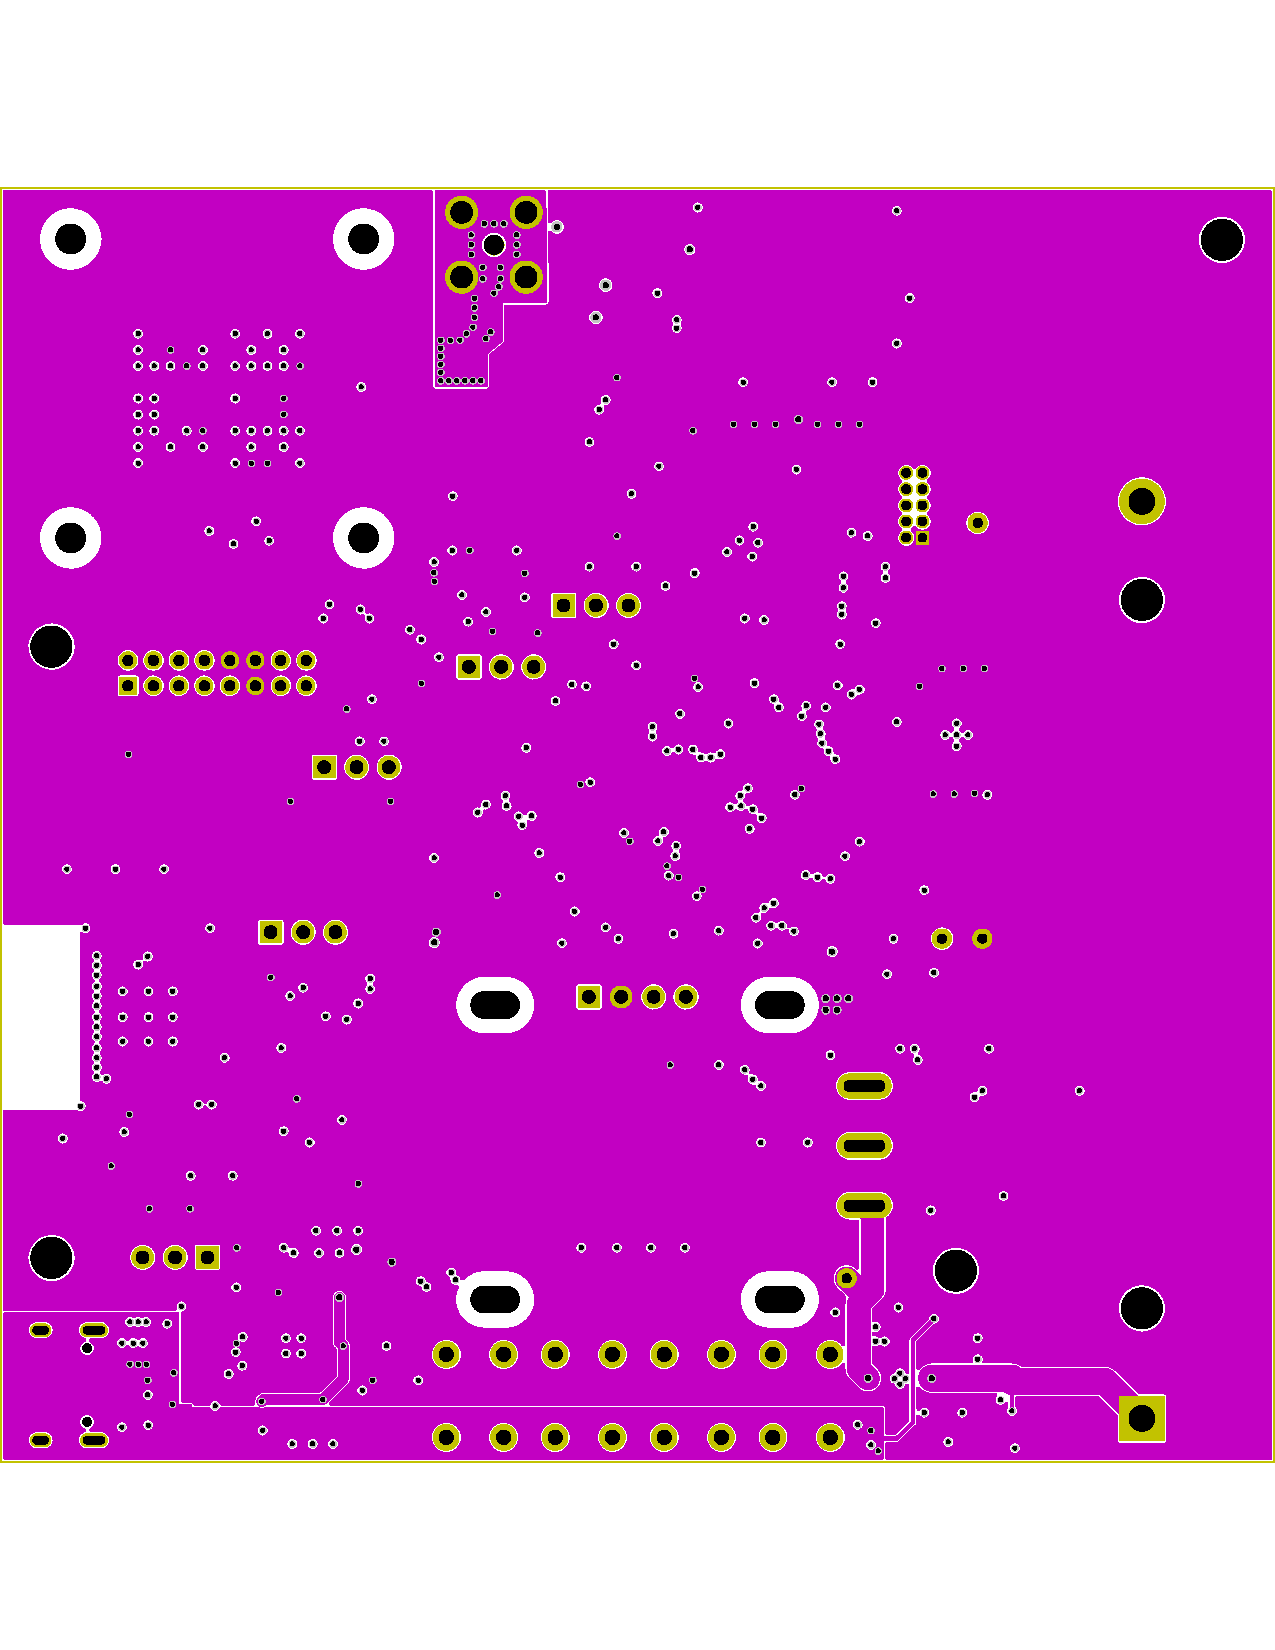
\includegraphics[width=\textwidth]{KiCad/boardIn2}

\section{Spodní vrstva mědi DPS} \label{BottomApp}
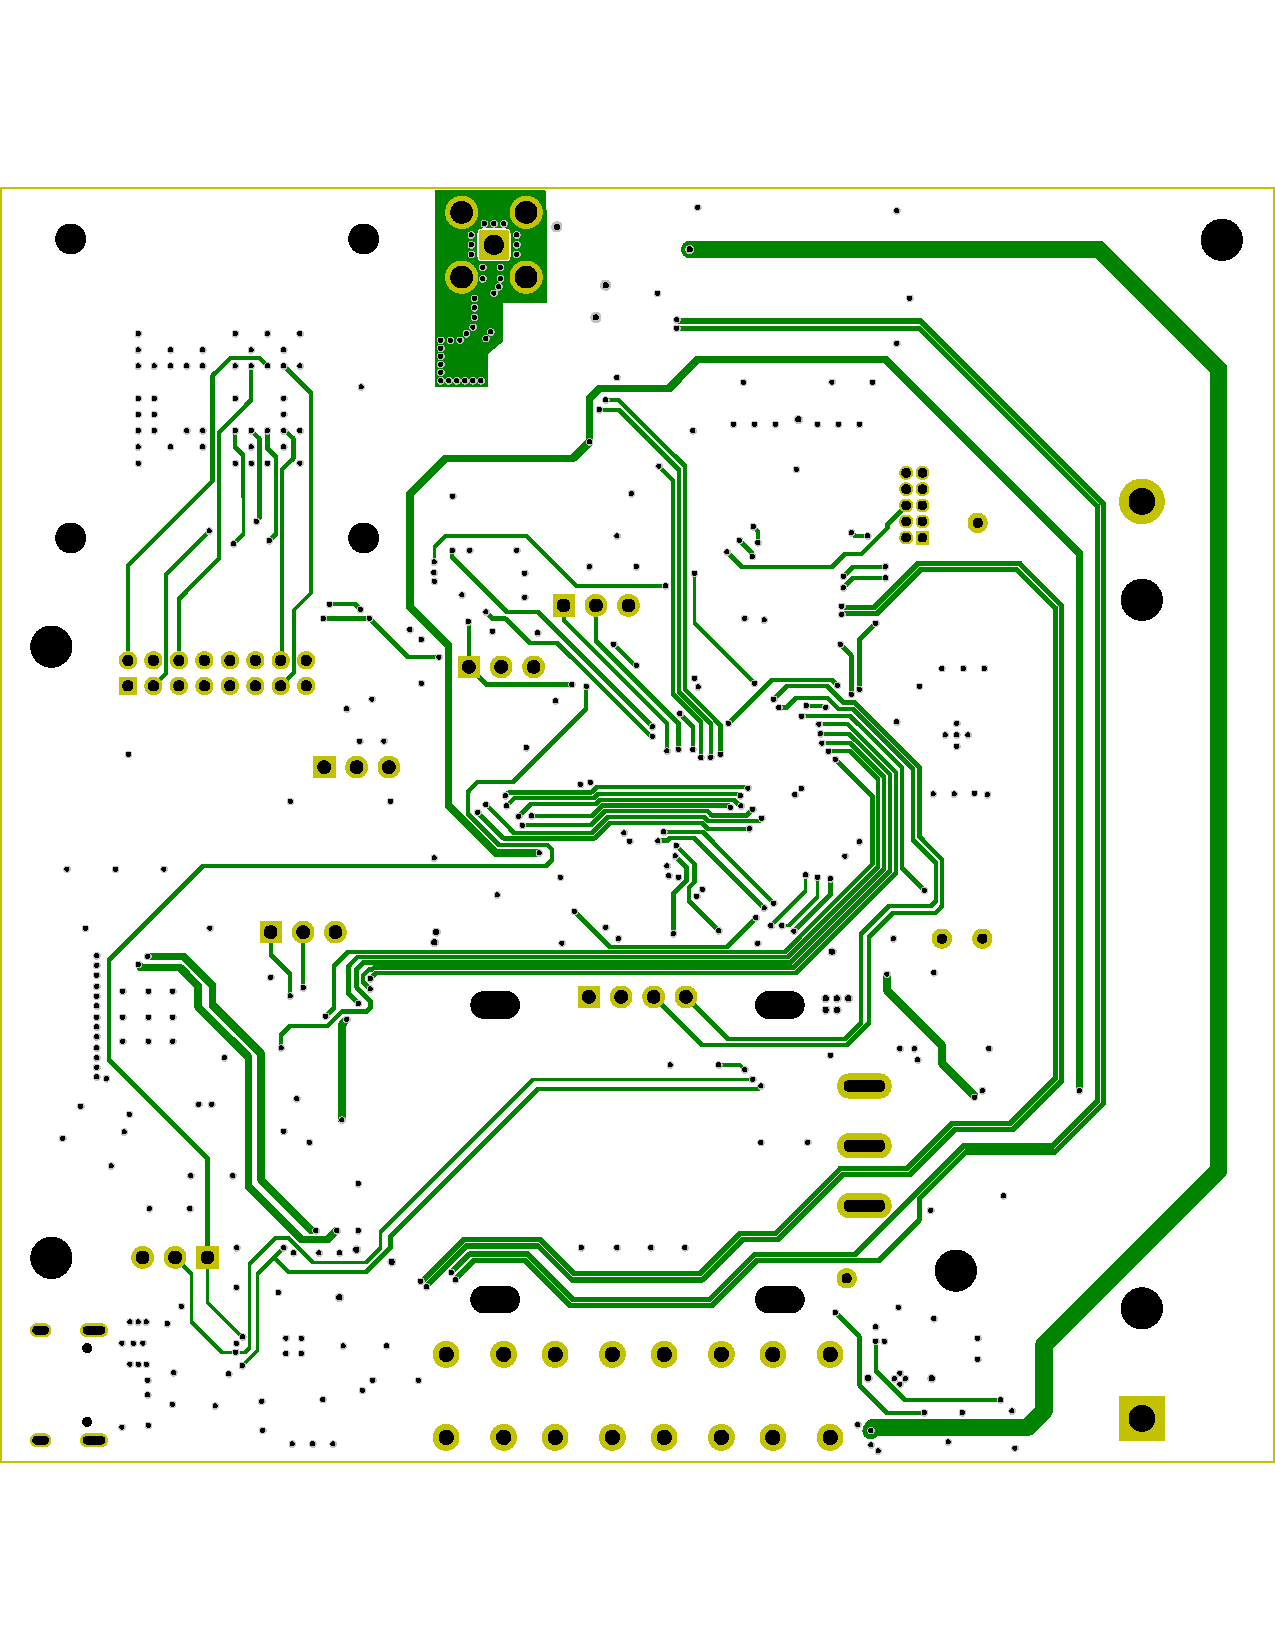
\includegraphics[width=\textwidth]{KiCad/boardB}


